\documentclass[a4paper,12pt]{article}
\usepackage[utf8]{inputenc}
\usepackage[polish]{babel}
\usepackage[OT4]{polski}

\usepackage{graphicx}
\graphicspath{ {images/} }

\title{Metody odktywania wiedzy\\\Large{Dokumentacja końcowa}}
\author{Rafał Okuniewski, Maciej Zaborek}
\date{czerwiec 2017}

\begin{document}

\maketitle

\section{Wstęp}
\section{Wstępne przetwarzanie danych}
\section{Algorytmy selekcji atrybutów}
	\subsection{Stepwise Regression}
		Final Model:
count ~ onwaytowork + hours + weekdays + windspeed + humidity + 
    atemp + workingday + season
	\subsection{Regsubset analisys}
		\begin{figure}[h]
   			\centering
    		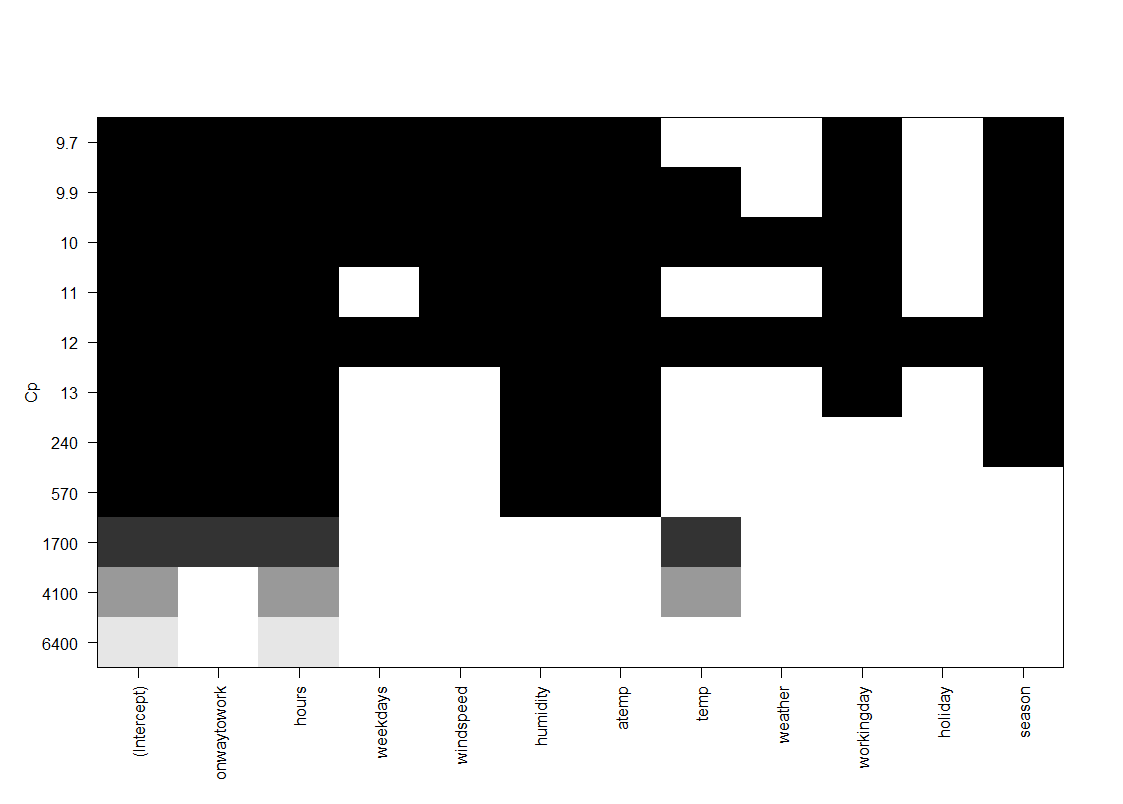
\includegraphics[width=\linewidth]{regsubsetanalysis}
		    \caption{Wyniki regsubset analisys}
    		\label{fig:my_label}
		\end{figure}
\section{Przetestowane algorytmy regresji}
    \subsection{Regresja liniowa}
		\begin{table}[h]
			\begin{tabular}{|p{2cm}|p{8cm}|r|r|}
				\hline 
				Liczba atrybutów & atrybuty & RMSLE & RMSE \\ 
				\hline 
				1 &  
				hours 
				&  
				1.328705
				&  
				152.3693
				\\ 
				\hline 
				2 &  
				hours + temp
				&  
				1.236916
				&  
				141.8473
				\\ 
				\hline 
				3 &  
				onwaytowork + hours + temp
				&  
				1.18398
				&  
				129.6105
				\\ 
				\hline 
				4 &  
				onwaytowork + hours + humidity + atemp
				&  
				1.172317
				&  
				123.351
				\\ 
				\hline 
				5 &  onwaytowork + hours + humidity + atemp + season 
				&  
				1.171745
				&  
				121.2109
				\\ 
				\hline 
				7 & onwaytowork + hours + windspeed + humidity + atemp + workingday + season &  
				1.152467
				&  
				119.855
				\\ 
				\hline 
				8 &  
				onwaytowork + hours + weekdays + windspeed + humidity + atemp + workingday + season  
				&  
				1.15163
				&  
				119.8403
				\\ 
				\hline 
			\end{tabular} 
			\caption{Błąd funkcji lm dla poszczególnych podzbiorów atrybutów zwróconych przez regsubset}
		\end{table}
	\subsection{Regresja lokalna}
		\begin{table}[h]
			\begin{tabular}{|c|c|c|c|}
				\hline 
				Degree & Span & RMSLE & RMSE \\ 
				\hline 
				2 & 0.01 & 0.78
				& 99.7 \\ 
				\hline 
				1 & 0.01 & 0.75 & 99.2 \\ 
				\hline 
				0 & 0.01 & 0.83 & 104 \\ 
				\hline 
				2 & 0.1 & 0.932 & 112 \\ 
				\hline 
				1 & 0.1 & 1 & 114 \\ 
				\hline 
				0 & 0.1 & 1.12 & 121 \\ 
				\hline 
				2 & 0.3 & 1.02 & 114 \\ 
				\hline 
				1 & 0.3 & 1.22 & 121 \\ 
				\hline 
				0 & 0.3 & 1.25 & 131 \\ 
				\hline 
				2 & 0.5 & 1.12 & 117 \\ 
				\hline 
				1 & 0.5 & 1.23 & 124 \\ 
				\hline 
				0 & 0.5 & 1.32 & 136 \\ 
				\hline 
				2 & 0.75 & 1.27 & 119 \\ 
				\hline 
				1 & 0.75 & 1.17 & 128 \\ 
				\hline 
				0 & 0.75 & 1.38 & 142 \\ 
				\hline 
				2 & 1 & 1.4 & 120 \\ 
				\hline 
				1 & 1 & 1.14 & 133 \\ 
				\hline 
				0 & 1 & 1.5 & 157 \\ 
				\hline 
			\end{tabular}
			\caption{Błąd funkcji loess w zależności od przyjętych parametrów dla formuły count \~ humidity + hours + atemp} 
		\end{table}
    \subsection{Robust regression z M-estymacją}
	\begin{table}    
    \begin{tabular}{|c|c|c|}
    \hline 
    Sposób estymacji & RMSLE & RMSE \\ 
    \hline 
    M-estymacja & 1.129622 & 120.9462 \\ 
    \hline 
    MM-estymacja & 1.110996 & 122.7891 \\ 
    \hline 
    \end{tabular}
    \caption{Wyniki w zależności od metody estymacji (średni błąd walidacji skrośnej dla k=5)}
    \end{table} 
    	\begin{table}
			\begin{tabular}{|c|c|c|}
				\hline 
				Funkcja psi & RMSLE & RMSE \\ 
				\hline 
				psi.bisquare & 1.116625 & 122.184 \\ 
				\hline 
				psi.huber & 1.129622 & 120.9462 \\ 
				\hline 
				psi.hampel & 1.14003 & 120.229 \\ 
				\hline 
		    \end{tabular}
		    \caption{Wyniki w zależności od funkcji psi}     
    	\end{table}
    	
    	\begin{table}
    		\begin{tabular}{|c|c|c|}
				\hline 
				& Dni robocze & Weekendy \\ 
				\hline 
				Robust RMSE & 120.8319 & 123.9919 \\ 
				\hline 
				Robust RMSLE & 1.034289 & 1.258234 \\ 
				\hline 
				Linear RMSLE & 1.097582 & 1.265375 \\ 
				\hline 
    		\end{tabular} 
    		\caption{dd}
    	\end{table}
    	
    	\begin{table}
    		\begin{tabular}{|c|c|c|}
				\hline 
				Liczba atrybutów & RMSLE & RMSE \\ 
				\hline 
				8 & 1.114278 & 122.9576 \\ 
				\hline 
				7 & 1.125025 & 140.3991 \\ 
				\hline 
				6 & 1.132462 & 137.4054 \\ 
				\hline 
				5 & 1.127936 & 138.382 \\ 
				\hline 
				4 & 1.137699 & 138.9563 \\ 
				\hline 
				3 & 1.129964 & 142.1899 \\ 
				\hline 
				2 & 1.190753 & 150.9452 \\ 
				\hline 
				1 & 1.22215 & 155.4499 \\ 
				\hline 
    		\end{tabular} 
    		\caption{dd}
    	\end{table}
    \subsection{Drzewa regresji}
		\begin{table}
			\begin{tabular}{|c|c|c|c|}
				\hline 
				Cp & Meth & RMSLE & RMSE \\ 
				\hline 
				0.005 & anova & 0.8742775 & 98.55746 \\ 
				\hline 
				0.01 & anova & 0.8742775 & 98.55746 \\ 
				\hline 
				0.01 & poisson & 0.7644792 & 100.8667 \\ 
				\hline 
				0.04 & anova & 0.9474914 & 124.1835 \\ 
				\hline 
				0.04 & poisson & 0.941012 & 123.5936 \\ 
				\hline 
				1 & anova & 0.9910873 & 135.782 \\ 
				\hline 
			\end{tabular} 
			\caption{dd}
		\end{table}
		
		\begin{table}
			\begin{tabular}{|c|c|c|}
				\hline 
				Liczba atrybutów & RMSLE & RMSE \\ 
				\hline 
				8 & 0.9396421 & 121.915 \\ 
				\hline 
				7 & 0.9301871 & 120.8053 \\ 
				\hline 
				6 & 0.9301871 & 120.8053 \\ 
				\hline 
				5 & 0.9596607 & 128.2725 \\ 
				\hline 
				4 & 0.9596607 & 128.2725 \\ 
				\hline 
				3 & 0.9596607 & 128.2725 \\ 
				\hline 
				2 & 0.9596607 & 128.2725 \\ 
				\hline 
				1 & 0.9596607 & 128.2725 \\ 
				\hline 
			\end{tabular} 
			\caption{dd}
		\end{table}
\section{Wnioski}

\end{document}
